%%%%%%%%%%%%%%%%%%%%%%%%%%%%%%%%%%%%%%%%%
% Beamer Presentation
% LaTeX Template
% Version 1.0 (10/11/12)
%
% This template has been downloaded from:
% http://www.LaTeXTemplates.com
%
% License:
% CC BY-NC-SA 3.0 (http://creativecommons.org/licenses/by-nc-sa/3.0/)
%
%%%%%%%%%%%%%%%%%%%%%%%%%%%%%%%%%%%%%%%%%

%----------------------------------------------------------------------------------------
%	PACKAGES AND THEMES
%----------------------------------------------------------------------------------------

\documentclass{beamer}

\mode<presentation> {

% The Beamer class comes with a number of default slide themes
% which change the colors and layouts of slides. Below this is a list
% of all the themes, uncomment each in turn to see what they look like.

%\usetheme{default}
%\usetheme{AnnArbor}
%\usetheme{Antibes}
%\usetheme{Bergen}
%\usetheme{Berkeley}
%\usetheme{Berlin}
%\usetheme{Boadilla}
%\usetheme{CambridgeUS}
%\usetheme{Copenhagen}
%\usetheme{Darmstadt}
%\usetheme{Dresden}
%\usetheme{Frankfurt}
%\usetheme{Goettingen}
%\usetheme{Hannover}
%\usetheme{Ilmenau}
%\usetheme{JuanLesPins}
%\usetheme{Luebeck}
\usetheme{Madrid}
%\usetheme{Malmoe}
%\usetheme{Marburg}
%\usetheme{Montpellier}
%\usetheme{PaloAlto}
%\usetheme{Pittsburgh}
%\usetheme{Rochester}
%\usetheme{Singapore}
%\usetheme{Szeged}
%\usetheme{Warsaw}

% As well as themes, the Beamer class has a number of color themes
% for any slide theme. Uncomment each of these in turn to see how it
% changes the colors of your current slide theme.

%\usecolortheme{albatross}
%\usecolortheme{beaver}
%\usecolortheme{beetle}
%\usecolortheme{crane}
%\usecolortheme{dolphin}
%\usecolortheme{dove}
%\usecolortheme{fly}
%\usecolortheme{lily}
%\usecolortheme{orchid}
%\usecolortheme{rose}
%\usecolortheme{seagull}
%\usecolortheme{seahorse}
%\usecolortheme{whale}
%\usecolortheme{wolverine}

%\setbeamertemplate{footline} % To remove the footer line in all slides uncomment this line
%\setbeamertemplate{footline}[page number] % To replace the footer line in all slides with a simple slide count uncomment this line

%\setbeamertemplate{navigation symbols}{} % To remove the navigation symbols from the bottom of all slides uncomment this line
}
\usepackage[brazil]{babel} % pacote portugues brasileiro
\usepackage[utf8]{inputenc} % pacote para acentuacao direta
\usepackage{graphicx} % Allows including images
\usepackage{booktabs} % Allows the use of \toprule, \midrule and \bottomrule in tables

%----------------------------------------------------------------------------------------
%	TITLE PAGE
%----------------------------------------------------------------------------------------

\title{Um Modelo Conceitual para Cenários de Acidentes em Atividades de Manutenção} % The short title appears at the bottom of every slide, the full title is only on the title page

\author{Jonathan M. Samara \\ Orientador Prof. Dr. Cesar A. Tacla} % Your name
\institute[UTFPR] % Your institution as it will appear on the bottom of every slide, may be shorthand to save space
{
Universidade Tecnológica Federal do Paraná \\ % Your institution for the title page
\medskip
}
\date{\today} % Date, can be changed to a custom date

\begin{document}

\begin{frame}
\titlepage % Print the title page as the first slide
\end{frame}

\begin{frame}
\frametitle{Introdução} % Table of contents slide, comment this block out to remove it
	\begin{itemize}
			\item \textbf{Motivação}: Averiguar e desenvolver modelos com base em sistemas multiagentes para aplicar em cenários de acidentes. 
			\item \textbf{Relevância}: Apresentar um modelo conceitual que defina em termos de classes e relacionamentos uma estrutura lógico-descritiva de fatores ambientais e organizacionais.    
	\end{itemize}
\end{frame}


\begin{frame}
\frametitle{Introdução - Objetivo Geral} % Table of contents slide, comment this block out to remove it
	\begin{itemize}
		\item \textbf{Sintetizar, construir e avaliar}, por intermédio de \textbf{observações, de análises de documentos técnicos, de análises de modelos computacionais} e de entrevista com profissionais da área, um modelo conceitual.
		\item Definir os \textbf{conceitos e as relações} para representar os cenários de ambientes de atividades, bem como os \textbf{respectivos acidentes que neles podem acontecer}.
		\item \textbf{Validar o processo} por verificar se os \textbf{raciocínios} (para um dado estudo de caso do setor de energia elétrica) resultantes desse modelo são correspondentes com a realidade a fim de levantar um entendimento formal do \textbf{problema para a comunidade acadêmica no que tange a que tipo de representação computacional} é mais apropriada para determinado contexto. 
	\end{itemize}
\end{frame}

\begin{frame}
\frametitle{Introdução - Objetivos Específicos}
	\begin{enumerate}
    	\item Identificar os aspectos relevantes que devem fazer parte da estrutura do modelo em relação aos 	riscos e consequências (acidentes) para os atores e atividades, que sejam relevantes na prática da 	atividade de manutenção, em caso de falha na operação. 
    	\item Construir um modelo conceitual que seja implementável computacionalmente e que produza as 	inferências que tratem aspectos relevantes ao problema.
    	\item Avaliar o modelo por aplicá-lo a um dado estudo de caso a fim de averiguar se os raciocínios 	produzidos nessa situação estão de acordo com a realidade.  
    	\item Analisar modelos computacionais em relação ao modelo conceitual desse estudo a fim de ter um 	levantamento formal do estado do problema. 
	\end{enumerate}
\end{frame}


\begin{frame}
\frametitle{Fundamentação Teórica - Agentes}
	\begin{itemize}
		\item Um agente é um sistema computacional autônomo. 
		\item Um artefato é uma entidade usada por um agente. 
		\item Um sistema multiagente é constituído por agentes autônomos que interagem visando um propósito em comum tendo como consequência um comportamento global.
		\item O aspecto normativo do sistema é tratado por considerar os eventos que resultam em uma violação e quais são as sanções decorrentes disso.
		\item BATU - \textit{Boundary Activities Tolerated during Use}
		\item BCTU - \textit{Boundary Condition Tolerated during Use} 				 
	\end{itemize}
\end{frame}


\begin{frame}
	\frametitle{Metodologia}
	\begin{minipage}[t]{0.48\linewidth}
		\begin{enumerate}
			\item \textbf{Revisão Exploratória e Análise de Campo}
			\begin{itemize}
				\item {\footnotesize Estudo de Manuais Técnicos}
				\item {\footnotesize Conversas com profissionais da área}
				\item {\footnotesize Entrevistas com Engenheiro de Manutenção}
				\item {\footnotesize Criação de Textos Descrevendo Cenários}
				\item {\footnotesize Participação de Workshops}
				\item {\footnotesize Acompanhamento de Procedimentos de Manutenção}
				\item {\footnotesize Revisão Bibliográfica}
			\end{itemize} 				
		\end{enumerate}
	\end{minipage}\hfill
	\begin{minipage}[t]{0.48\linewidth}
		\begin{enumerate}
			\item \textbf{Formalização de um Modelo Conceitual}
			\begin{itemize}
				\item {\footnotesize Identificar Padrões}
				\item {\footnotesize Formalizar em termos de Conceitos e Relações}
			\end{itemize}			 
			\item \textbf{Explorar os Arcabouços Possíveis}
			\begin{itemize}
				\item {\footnotesize Avaliar correspondência com outros Arcabouços}
   			\end{itemize}			 
			\item \textbf{Aplicação em Estudo de Caso}
			\begin{itemize}
				\item {\footnotesize Modelar um dado estudo de caso no modelo obtido}
				\item {\footnotesize Analisar os raciocínios decorrentes frente a realidade}
   			\end{itemize}			 
		\end{enumerate}
	\end{minipage}	 
\end{frame}

\begin{frame}
	\frametitle{Resultados - Revisão Exploratória e Análise de Campo}
	\begin{enumerate}
		\item {Os trabalhadores que executam os procedimentos.}
		\item {Os diferentes papéis (ou funções) desses trabalhadores.}
		\item {As ferramentas usadas pelos profissionais.}
		\item {Os equipamentos que são submetidos a manutenção.}
		\item {As interações entre todo tipo de entidade tais como trabalhadores, ferramentas e equipamentos.}
		\item {As etapas das tarefas que devem ser finalizadas.}
		\item {As relações entre todas as entidades e interações com as tarefas.} 			
	\end{enumerate}
\end{frame}

\begin{frame}
	\frametitle{Resultados - Revisão Exploratória e Análise de Campo}
	\begin{enumerate}
		\item { Averiguar a incerteza presente em certos processos e equipamentos que podem gerar acidentes.}
		\item { Análise das Medidas que são tomadas pelos profissionais para lidar com essas incertezas.}
		\item { Análise de Cenários onde Profissionais tomam medidas em desacordo com a segurança.}
		\item { Análise dos riscos gerados a todos.}
		\item { Análise da possibilidade de algum acidente ocorrer.}
	\end{enumerate}
\end{frame}


\begin{frame}
	\frametitle{Resultados - Revisão Exploratória e Análise de Campo}
 	\begin{enumerate}
		\item MOISE+
		\begin{itemize}
		 	\item HuBNER, J.; SICHMAN, J.; BOISSIER, O. Moise+: Towards a structural, functional, and deontic model for mas organization. In: . [S.l.: s.n.], 2002. p. 501–502., 
			\item HuBNER, J. F.; SICHMAN, J. S.; BOISSIER, O. A model for the structural, functional, and deontic specification of organizations in multiagent systems. In: BITTENCOURT, G.; RAMALHO, G. L. (Ed.). Advances in Artificial Intelligence. Berlin, Heidelberg: Springer Berlin Heidelberg, 2002. p. 118–128. ISBN 978-3-540-36127-5.
		\end{itemize}
		\item Modelo de Agentes Normativos de Dastani
		\begin{itemize}
			\item DASTANI, M. et al. Normative multi-agent programs and their logics. In: MEYER, J.-J. C.; BROERSEN, J. (Ed.). Knowledge Representation for Agents and Multi-Agent Systems. Berlin, Heidelberg: Springer Berlin Heidelberg, 2009. p. 16–31. ISBN 978-3-642-05301-6.
		\end{itemize}
	\end{enumerate}
\end{frame}

\begin{frame}
	\frametitle{Resultados - Revisão Exploratória e Análise de Campo}
 	\begin{enumerate}
		\item V3S
		\begin{itemize}
			\item BAROT, C. et al. V3S: A virtual environment for risk-management training based on human-activity models. Presence, v. 22, n. 1, p. 1–19, 2013.
		\end{itemize}
		\item NormMAS
		\begin{itemize}
			\item CHANG, S.; MENEGUZZI, F. Simulating normative behaviour in multi-agent environments using monitoring artefacts. In: DIGNUM, V. et al. (Ed.). Coordination, Organizations, Institutions, and Norms in Agent Systems XI. Cham: Springer International Publishing, 2016. p. 59–77. ISBN 978-3-319-42691-4.
		\end{itemize}

	\end{enumerate}
\end{frame}


\begin{frame}
	\frametitle{Resultados - Estrutural Conceitual - Módulos}
	\begin{figure}[H]
  		\centering
  			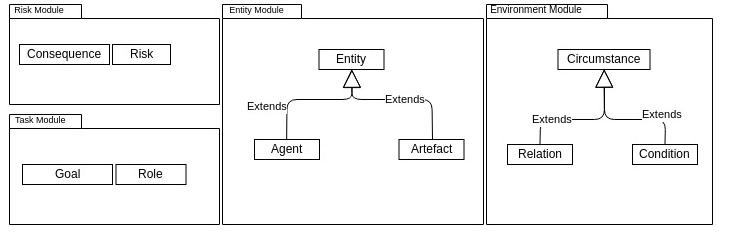
\includegraphics[width=1\linewidth]{../dissertacao/figure/Module.jpeg} 
  		\caption{A estrutura geral das classes do modelo}
  		\label{module}
	\end{figure}
\end{frame}

\begin{frame}
	\frametitle{Resultados - Estrutural Conceitual - Predicados}
	\begin{figure}[H]
  		\centering
  		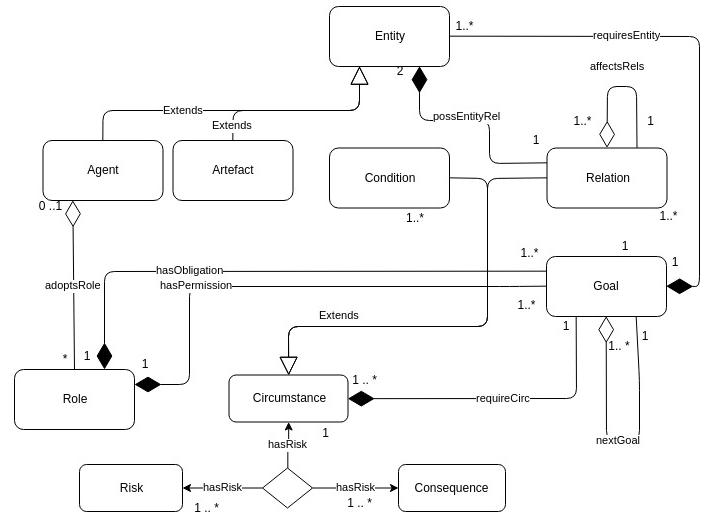
\includegraphics[width=0.8\linewidth]{../dissertacao/figure/Class.jpeg} 
  		\caption{Diagrama de classes do Modelo}
  		\label{classdiagrama}
	\end{figure}
\end{frame}

\begin{frame}
	\frametitle{Resultados - Regras}
	\begin{eqnarray}\label{violationrelation}\nonumber
		hasObligation(\rho_m,g_j) \to hasPermission(\rho_m,g_j), \nonumber \\
    	\rho_m \in Role \wedge g_j \in Goal
	\end{eqnarray}
	\begin{eqnarray}\label{violationentity}\nonumber
		requiresCirc(g_i,c_k) \wedge \neg isPresent(c_k) \wedge  instanceOfCond(c_k) \nonumber \\ 
		\wedge  starts(ag_m,g_i)  \to conditionViol(ag_m,g_i,c_k) \nonumber \\  
    	g_i \in Goal, c_k \in Condition, ag_m \in Agent
	\end{eqnarray}
	\begin{eqnarray}\label{relationViol}\nonumber
		requiresCirc(g_i,r_k)\wedge \neg isPresent(r_k) \wedge instanceOfRel(r_k) \nonumber \\ 
		\wedge starts(ag_m,g_i) \to relationViol(ag_m,g_i,r_k) \nonumber \\  
    	g_i \in Goal, r_k \in Relation, ag_m \in Agent
	\end{eqnarray}
	\begin{eqnarray}\label{entityViol}\nonumber
		requiresEntity(g_i,eg_n) \wedge \neg isPresent(e_k) \wedge starts(ag_m,g_i) \to \nonumber \\ 
	    entityViol(ag_m,g_i,e_k)  \nonumber \\  
	    g_i \in Goal, e_k \in Entity, ag_m \in Agent
	\end{eqnarray}
\end{frame}
\begin{frame}
	\frametitle{Resultados - Regras}
	\begin{eqnarray}\label{consconditionViol}\nonumber
		conditionViol(ag_m,g_i,c_k)  \wedge hasRisk(c_k,risk_j,cs_m) \to \nonumber \\ 
		negConseqFor(g_i,ag_m,risk_j,cs_m) \nonumber \\ 
    	ag_m \in Agent, g_i \in Goal, c_k \in Condition, risk_k \in Risk, cs_m \in Consequence
	\end{eqnarray}
	\begin{eqnarray}\label{consrelationViol}\nonumber
		relationViol(ag_m,g_i,r_k) \wedge hasRisk(r_k,risk_j,cs_m) \to \nonumber \\ 
		negConseqFor(g_i,ag_m,risk_j,cs_m) \nonumber \\ 
	    ag_m \in Agent, g_i \in Goal, r_k \in Relation, risk_k \in Risk, cs_m \in Consequence 
	\end{eqnarray}
	\begin{eqnarray}\label{entityViolaffect}
		relationViol(ag_m,g_i,r_k) \wedge affectsRels(r_k,r_n) \to possOfNegConseqFor(r_n)  \nonumber \\
	    ag_m \in Agent, g_i \in Goal, r_k,r_n \in Relation, 
	\end{eqnarray}
	\begin{eqnarray}\label{consvioent}
		entityViol(ag_m,g_i,e_k) \to stopped(g_i) \nonumber \\  
    	ag_m \in Agent, g_i \in Goal, e_k \in Entity \\ \nonumber
	\end{eqnarray}
\end{frame}

\begin{frame}
	\frametitle{Resultados - Regras}
	\begin{eqnarray}\label{paybutiamnotguilty}
		possOfNegConseqFor(r_k) \wedge  happensNegConseqFor(r_k) \wedge \nonumber \\
		requiresCirc(g_i,r_k) \wedge instanceOfRel(r_k) \wedge \nonumber \\ 
		hasRisk(r_k,risk_j,cs_m) \wedge starts(ag_m,g_i) \nonumber \\ 
		\to negConseqFor(g_i,ag_m,risk_j,cs_m) \nonumber \\ 
	    r_k \in Relation, g_i \in Goal, risk_k \in Risk, cs_m \in Consequence
	\end{eqnarray}
	 \begin{eqnarray}\label{badcons}
		negConseqFor(g_k,ag_m,risk_j,cs_m) \to stopped(g_k) \nonumber \\ 
	    g_k \in Goal, risk_j \in Risk, cs_m \in Consequence
	\end{eqnarray}	
\end{frame}

\begin{frame}
	\frametitle{Resultados - Regras}
	\begin{eqnarray}\label{rolenextgoal}
		adoptsRole(ag_n,\rho_m) \wedge hasPermission(\rho_m,g_j) \wedge nextGoal(g_i,g_j) \nonumber \\
	 	\wedge reached(g_i) \to enabledToStart(ag_i,g_j) \nonumber \\
    	ag_i, ag_n \in Agent, \rho_m \in Role, g_j \in Goal, g_i \in Goal
	\end{eqnarray}
	\begin{eqnarray}\label{rolelastgoal}
		adoptsRole(ag_n,\rho_m) \wedge hasPermission(\rho_m,g_i) \wedge lastGoal(g_i,\rho_m) \nonumber \\
		\wedge reached(g_i) \to stopped(g_i) \nonumber \\
		ag_n \in Agent, \rho_m \in Role, g_i \in Goal
	\end{eqnarray}
\end{frame}
\begin{frame}
	\frametitle{Resultados - Regras}
	\begin{figure}[H]
		\centering
		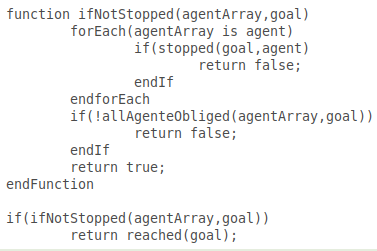
\includegraphics[width=0.6\linewidth]{../dissertacao/figure/algrule6.png} 
		\caption{Condição para definir se um dado objetivo foi atingido ou não} \label{wenStop}  
	\end{figure}
\end{frame}

\begin{frame}
	\frametitle{Resultados - Estudo de Caso}
	\begin{itemize}
		\item O estudo de caso desta pesquisa consiste em sete profissionais de linha viva.
		\item Um supervisor e seis executores.
		\item Céu ensolarado e umidade relativa do ar menor que 70 porcento.
		\item EPI's necessários: capacete, óculos de sol, roupa isolante e antichamas, luvas isolantes e botas isolantes.
		\item  bastão garra de diâmetro 64 x 3600 mm, sela de diâmetro 65, colar, corda de fibra sintética, carretilha, chave com catraca, bastão universal, soquete adequado, locador de pino e bastão com soquete multiangular
		\item O método selecionado para esse tipo de manutenção é a distância.
	\end{itemize}
\end{frame}
\begin{frame}
	\frametitle{Resultados - Raciocínio 1}
	\begin{enumerate}
		\item $adoptsRole(agente4,executor2)$ 
		\item $hasObligation(executor2,g1)$
		\item $requiresCirc(g1,relPanoGlicerina)$
		\item $instanceOfRel(relPanoGlicerina)$ 
		\item $\neg isPresent(relPanoGlicerina)$
		\item $starts(agente4,g1)$
		\item $affectsRels(relPanoGlicerina,relBastaoGarraCondutor)$
		\item $affectsRels(relPanoGlicerina,relCordaEstropo)$  
		\item $affectsRels(relPanoGlicerina,relChaveCatracaParafuso)$
		\item $affectsRels(relPanoGlicerina,relParafusoConector)$ 
		\item $affectsRels(relPanoGlicerina,relSoqueteParafuso)$ 
		\item $affectsRels(relPanoGlicerina,relAgente4Corda)$ 
		\item $affectsRels(relPanoGlicerina,relEstropoCorda)$	
	\end{enumerate}
\end{frame}
\begin{frame}
	\frametitle{Resultados - Raciocínio 1}
	\begin{eqnarray}\nonumber
		requiresCirc(g1,relPanoGlicerina) \wedge \nonumber \\  
		\neg isPresent(relPanoGlicerina) \wedge \nonumber \\   
		instanceOfRel(relPanoGlicerina) \wedge \nonumber \\   
		starts(agente4,g1) \to \nonumber \\
		relationViol(agente4,g1,relPanoGlicerina) \nonumber \\  
	\end{eqnarray}
	\begin{eqnarray} \nonumber
		relationViol(agente4,g1,relPanoGlicerina) \nonumber \\
		\wedge affectsRels(relPanoGlicerina,relEstropoCorda) \nonumber \\
    	\to possOfNegConseqFor(relEstropoCorda) \nonumber \\
	\end{eqnarray}

	O mesmo ocorre para as demais relações.
\end{frame}
\begin{frame}
	\frametitle{Resultados - Raciocínio 2}
	\begin{enumerate}
		\item $adoptsRole(agente2,executor1)$ 
		\item $adoptsRole(agente3,executor1)$	 	
		\item $adoptsRole(agente4,executor2)$	 
		\item $hasObligation(executor1,g1)$
		\item $hasObligation(executor2,g1)$
		\item $starts(agente2,g1)$ 
		\item $starts(agente3,g1)$	 	
		\item $starts(agente4,g1)$	
		\item $requiresEntity(g1,pano)$		
		\item $\neg isPresent(pano)$
	\end{enumerate}
\end{frame}
\begin{frame}
	\frametitle{Resultados - Raciocínio 2}
	\begin{eqnarray}\nonumber
		requiresEntity(g1,pano) \wedge \neg isPresent(pano) \wedge starts(agente2,g1)  \nonumber \\ 
		\to entityViol(agente2,g1,pano) \nonumber \\ 	    
	\end{eqnarray}

	\begin{eqnarray}\nonumber
		requiresEntity(g1,pano) \wedge \neg isPresent(pano) \wedge starts(agente3,g1) \nonumber \\ 
	    \to entityViol(agente3,g1,pano) \nonumber \\
	\end{eqnarray}
	\begin{eqnarray}\nonumber
		requiresEntity(g1,pano) \wedge \neg isPresent(pano) \wedge starts(agente4,g1) \nonumber \\ 
	    \to entityViol(agente4,g1,pano)  \nonumber \\	
	\end{eqnarray}
	\begin{eqnarray}
		entityViol(agente4,g1,pano) \to stopped(g1)
	\end{eqnarray}
\end{frame}

\begin{frame}
	\frametitle{Resultados - Raciocínio 3}
	\begin{enumerate}
		\item $adoptsRole(agente5,executor3)$
		\item $hasObligation(executor3,g11)$	
		\item $starts(agente5,g11)$ 
		\item $requiresCirc(g11,umidade70)$
		\item $isIstanceOfCond(umidade70)$
		\item $\neg isPresent(umidade70)$
		\item $hasRisk(umidade70,eletrocutado,morte)$
	\end{enumerate}
\end{frame}

\begin{frame}
	\frametitle{Resultados - Raciocínio 3}
	\begin{eqnarray}\nonumber
		requiresCirc(g11,umidade70) \wedge \neg isPresent(umidade70) \\ \nonumber
		\wedge instanceOfCond(umidade70) \wedge starts(agente5,g11)  \to \\ \nonumber   
		conditionViol(agente5,g11,umidade70) \nonumber \\	
	\end{eqnarray}
	\begin{eqnarray} \nonumber
		conditionViol(agente5,g11,umidade70) \wedge \nonumber \\
		hasRisk(umidade70,eletrocutado,morte) \nonumber \\ 
		\to negConseqFor(g11,agente5,eletrocutado,morte) \nonumber \\ 	
	\end{eqnarray}
	\begin{eqnarray}
		negConseqFor(g11,agente5,eletrocutado,morte) \to stopped(g11)
	\end{eqnarray}

\end{frame}

\begin{frame}
	\frametitle{Resultados - Raciocínio 4}
	\begin{enumerate}
		\item $adoptsRole(agente4,executor2)$
		\item $hasObligation(executor4,g15)$	
		\item $starts(agente4,g15)$ 
		\item $requiresCirc(g15,relChaveCatracaParafuso)$
		\item $isInstanceOfRel(relChaveCatracaParafuso)$	
		\item $\neg isPresent(relChaveCatracaParafuso)$
		\item $hasRisk(relChaveCatracaParafuso,eletrocutado,morte)$
	\end{enumerate}
\end{frame}

\begin{frame}
	\frametitle{Resultados - Raciocínio 4}
	\begin{eqnarray} \nonumber
		requiresCirc(g15,relChaveCatracaParafuso)\wedge  \nonumber \\
		\neg isPresent(relChaveCatracaParafuso) \wedge \nonumber \\
		instanceOfRel(relChaveCatracaParafuso) \wedge starts(agente4,g15) \to \nonumber \\
		relationViol(agente4,g15,relChaveCatracaParafuso)
	\end{eqnarray}
	\begin{eqnarray}\nonumber
		relationViol(agente4,g15,relChaveCatracaParafuso) \nonumber \\ 
		 \wedge hasRisk(relChaveCatracaParafuso,eletrocutado,morte) \to \nonumber \\ 
		negConseqFor(g15,agente4,eletrocutado,morte)
	\end{eqnarray}	
	\begin{eqnarray}
		negConseqFor(g15,agente4,eletrocutado,morte) \to stopped(g15)
	\end{eqnarray}
\end{frame}

\begin{frame}
	\frametitle{Resultados - Raciocínio 5}
	\begin{enumerate}
		\item $requiresCirc(g19,relParafusoConector)$		
		\item $hasObligation(executor3,g19)$
		\item $hasObligation(executor4,g19)$
		\item $hasObligation(executor5,g19)$		
		\item $starts(agente5,g19)$
		\item $starts(agente6,g19)$
		\item $starts(agente7,g19)$									
		\item $adoptsRole(agente5,executor3)$
		\item $adoptsRole(agente6,executor4)$
		\item $adoptsRole(agente7,executor5)$
		\item $hasRisk(relParafusoConector,eletrocutado,morte)$
		\item $possOfNegConseqFor(relParafusoConector)$
		\item $happensNegConseqFor(g19,relParafusoConector)$	
	\end{enumerate}
\end{frame}

\begin{frame}
	\frametitle{Resultados - Raciocínio 5}
	\begin{eqnarray}\nonumber
	   possOfNegConseqFor(relParafusoConector) \nonumber \\
	    \wedge happensNegConseqFor(relParafusoConector) \nonumber \\ 
	    \wedge requiresCirc(g19,relParafusoConector) \nonumber \\  
	    \wedge instanceOfRel(relParafusoConector) \nonumber \\ 
	    \wedge hasRisk(relParafusoConector,eletrocutado,morte) \nonumber \\  
	    \wedge starts(agente5,g19) \nonumber \\ 
	    \to negConseqFor(g19,agente5,eletrocutado,morte) \\ \nonumber    
	\end{eqnarray}	
	\begin{eqnarray}
		negConseqFor(g19,agente5,eletrocutado,morte) \to stopped(g19)
	\end{eqnarray}
	O mesmo para o agente6 e agente7.
\end{frame}

\begin{frame}
	\frametitle{Resultados - Raciocínio 6}
	\begin{enumerate}
		\item $stopped(agente2,g23) \to F$	
		\item $stopped(agente3,g23) \to F$
		\item $stopped(agente4,g23) \to F$
		\item $stopped(agente5,g23) \to F$
		\item $stopped(agente7,g23) \to F$
		\item $hasObligation(executor1,g23)$	
		\item $hasObligation(executor2,g23)$	
		\item $hasObligation(executor3,g23)$		
		\item $adoptsRole(agente2,executor1)$
		\item $adoptsRole(agente3,executor1)$
		\item $adoptsRole(agente4,executor2)$
		\item $adoptsRole(agente5,executor3)$
		\item $adoptsRole(agente7,executor5)$
	\end{enumerate}
\end{frame}
\begin{frame}
	\frametitle{Resultados - Raciocínio 6}
	\begin{itemize}
		\item $ag_{array} = \{ agente2,agente3,agente4,agente5,agente7 \}$
		\item $stopped(goal,Agente) \to F$ para todos os agentes		
		\item $allAgentObligate(ag_{array},goal) \to T$
		\item $ifNotStopped(ag_{array},goal) \to T$
		\item $reached(goal) \to T$
	\end{itemize}
\end{frame}
\begin{frame}
	\frametitle{Discussão - Critérios de Comparação}
	\begin{itemize}
		\item \textbf{Agente} condiz numa representação dos estados internos que um agente pode ter
		\item O critério \textbf{SMA} condiz na presença de elementos que são necessários para especificar um \textit{Sistema Multiagente}
		\item O critério \textbf{Artefato} condiz com elementos que correspondem ao tratado na Fundamentação Teórica.
		\item \textbf{Norma} corresponde a regras que devem ser acatadas pelos agentes 
		\item \textbf{Violação} define o que corresponde o não cumprimento de uma dada regra
		\item \textbf{Sanção} implica penalidade sobre o agente.
		\item \textbf{Risco} implica o evento ruim que tem um dado potencial de ocorrer sobre o agente
	\end{itemize}
\end{frame}
\begin{frame}
	\frametitle{Discussão - Critérios de Comparação}
	\begin{itemize}
		\item \textbf{P.O.A.E} significa Possibilidade de Ocorrer algo Errado.
		\item \textbf{Objetivos} implica alvos que devem ser atingidos pelos agentes 
		\item \textbf{C.A} consiste em condições ambientes que interagem com a atividade executada pelos agentes.
		\item \textbf{I.AG.AR} representa as interações entre agentes e artefatos
		\item \textbf{D.C.A} - Descrição de Cenários de Acidentes, consiste na capacidade de desenvolver raciocínios a fim de representar cenários de acidentes.
	\end{itemize}
\end{frame}

\begin{frame}
	\frametitle{Discussão - Análise Comparativa}
	\begin{figure}[H]
		\centering
		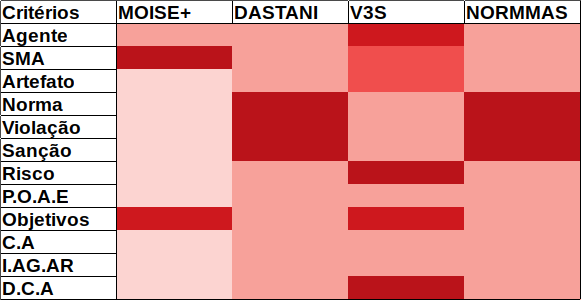
\includegraphics[width=1\linewidth]{figure/table_head.png} 
		\label{classdiagrama}
	\end{figure}
\end{frame}

\begin{frame}
	\frametitle{Discussão - Consistência dos Resultados - Estudo de Caso}
	\begin{itemize}
		\item  O caso em análise cumpre com os interesses da pesquisa pois apresenta um cenário onde profissionais usam ferramentas para trabalhar de forma colaborativa a fim de atingir um determinado objetivo
		\item Os profissionais são expostos a um dado risco e podem sofrer acidentes que advêm tanto de responsabilidade própria bem como responsabilidade do outro.
		\item O estudo de caso em análise é um cenário que é totalmente possível de ser factual, contudo existe diversas outras possibilidades de organizar a mesma manutenção.
	\end{itemize}
\end{frame}

\begin{frame}
	\frametitle{Discussão - Considerações sobre Critérios Metodológicos ao Estudo de Caso}
	\begin{itemize}
		\item Organização dos Objetivos pode ser modificada pelos profissionais durante a execução das Atividades.		
		\item Não se considera todos os riscos, mas os mais prováveis.
		\item $affectsRels(r_k,r_n)$ - simplifica o processo de modelagem.
		\item $possEntityRel(r_l,e_i,e_k)$ - granulidade do modelo.
		\item $requiresCirc(circ_n,g_m)$, $requiresEntity(goal_i, e_j)$, $instanceOfRel(circ_n)$ e $instanceOfCond(circ_n)$ - granulidade do modelo. 
	\end{itemize}
\end{frame}

\begin{frame}
	\frametitle{Discussão - Considerações sobre Critérios Metodológicos ao Raciocínios}
	\begin{itemize}
		\item Raciocínio 1 e 5  - Cenário de violação de relação sem sanção.  
		\item Raciocínio 2 - Violação de Entidade 
		\item Raciocínio 3 - Violação de Condição
		\item Raciocínio 4 - Violação de Relação com Sanção
		\item Raciocínio 6 - Atingiu o objetivo
	\end{itemize}
\end{frame}


\begin{frame}
	\frametitle{Conclusão - Reflexão sobre Objetivo}
	\begin{itemize} 
		\item Foi feito estudo de documentos técnicos, foi feito entrevista com Engenheiro de Manutenção, foi feito acompanhamento de documentos técnicos, houve acompanhamento de procedimentos de manutenção em linha viva.
		\item Foi concebido um modelo conceitual.
		\item O modelo conceitual foi aplicado em um estudo de caso. Isso possibilitou formular raciocínios e verificar quais cenários foram representados apropriadamente e quais cenários não foram representados adequadamente.
		\item Houve uma análise da comparativa entre modelos computacionais balizado pelo modelo conceitual definido nesse estudo.
		\item Logo, o Objetivo Geral e os Objetivos Específicos foram atingidos.    
	\end{itemize}
\end{frame}

\begin{frame}
	\frametitle{Conclusão}
	\begin{itemize}
		\item \textit{MOISE+} é mais apropriado para representar os seguintes conceitos: \textit{Agente, SMA, objetivos};
		\item \textit{Dastani} é mais apropriado para representar os seguintes conceitos \textit{Normas, Violações, Sanções};
		\item \textit{V3S} é mais apropriado para representar \textit{SMA, Artefato, Riscos e contém estruturas otimizadas para descrever dinamicamente os cenários de acidentes}
		\item \textit{NORMMAS} é mais apropriado para representar os seguintes conceitos \textit{Normas, Violações, Sanções};
		\item No que tange ao contraste do modelo conceitual proposto nesse estudo em relação aos arcabouços verificados nesse texto, o autor conclui que aquele unifica em uma única estrutura concepções que são tratadas de formas isoladas aos demais modelos computacionais.
	\end{itemize}
\end{frame}

\begin{frame}
	\frametitle{Conclusão}
	\begin{enumerate}
		\item Em vez de trabalhar conceitos de possibilidade, sintetizar um modelo estatístico probabilístico na estrutura conceitual proposta neste estudo.
		\item Investigar novas estruturas conceituais para tratar cenários onde os agentes buscam técnicas alternativas para resolver um determinado problema. 
		\item Investigar novas estruturas conceituais onde uma violação pode ou não gerar uma sanção para as condições ambientes (ou seja, em vez de tratar a possibilidade sobre um relacionamento futuro, tratar a possibilidade sobre um relacionamento presente).
		\item Investigar novas estruturas conceituais que considerem a violação de relacionamento em termos de possibilidades e não de um efeito direto no que tange a uma dada causa.   
	\end{enumerate}
\end{frame}


\end{document} 	